\subsubsection{Estrategia de Exploración Sistemática}

El robot debe construir una representación espacial completa del entorno de cultivo para identificar todas las estaciones que contienen lechugas disponibles para cosecha. Esta tarea se aborda mediante una estrategia de exploración sistemática que aprovecha la geometría estructurada del sistema hidropónico.

El sistema de cultivo consiste en tubos horizontales de PVC dispuestos paralelamente con separación uniforme de 200 milímetros entre centros. Cada tubo contiene estaciones de cultivo separadas 150 milímetros entre sí. El área total de trabajo es de 1800 milímetros en dirección horizontal (eje X) y 1200 milímetros en dirección vertical (eje Y), resultando en un total de 72 estaciones distribuidas en 6 filas de 12 estaciones cada una.

La estrategia de exploración implementada sigue un patrón de barrido tipo serpiente que minimiza los movimientos en el eje vertical, que presenta velocidad significativamente menor que el eje horizontal. El robot inicia en la esquina inferior izquierda del espacio de trabajo (coordenada 0,0) y recorre la primera fila completa en dirección positiva de X. Al alcanzar el extremo derecho, incrementa su posición en Y para pasar a la segunda fila, que recorre en dirección negativa de X (de derecha a izquierda). Este patrón alternado se repite hasta completar todas las filas.

\begin{figure}[h]
\centering
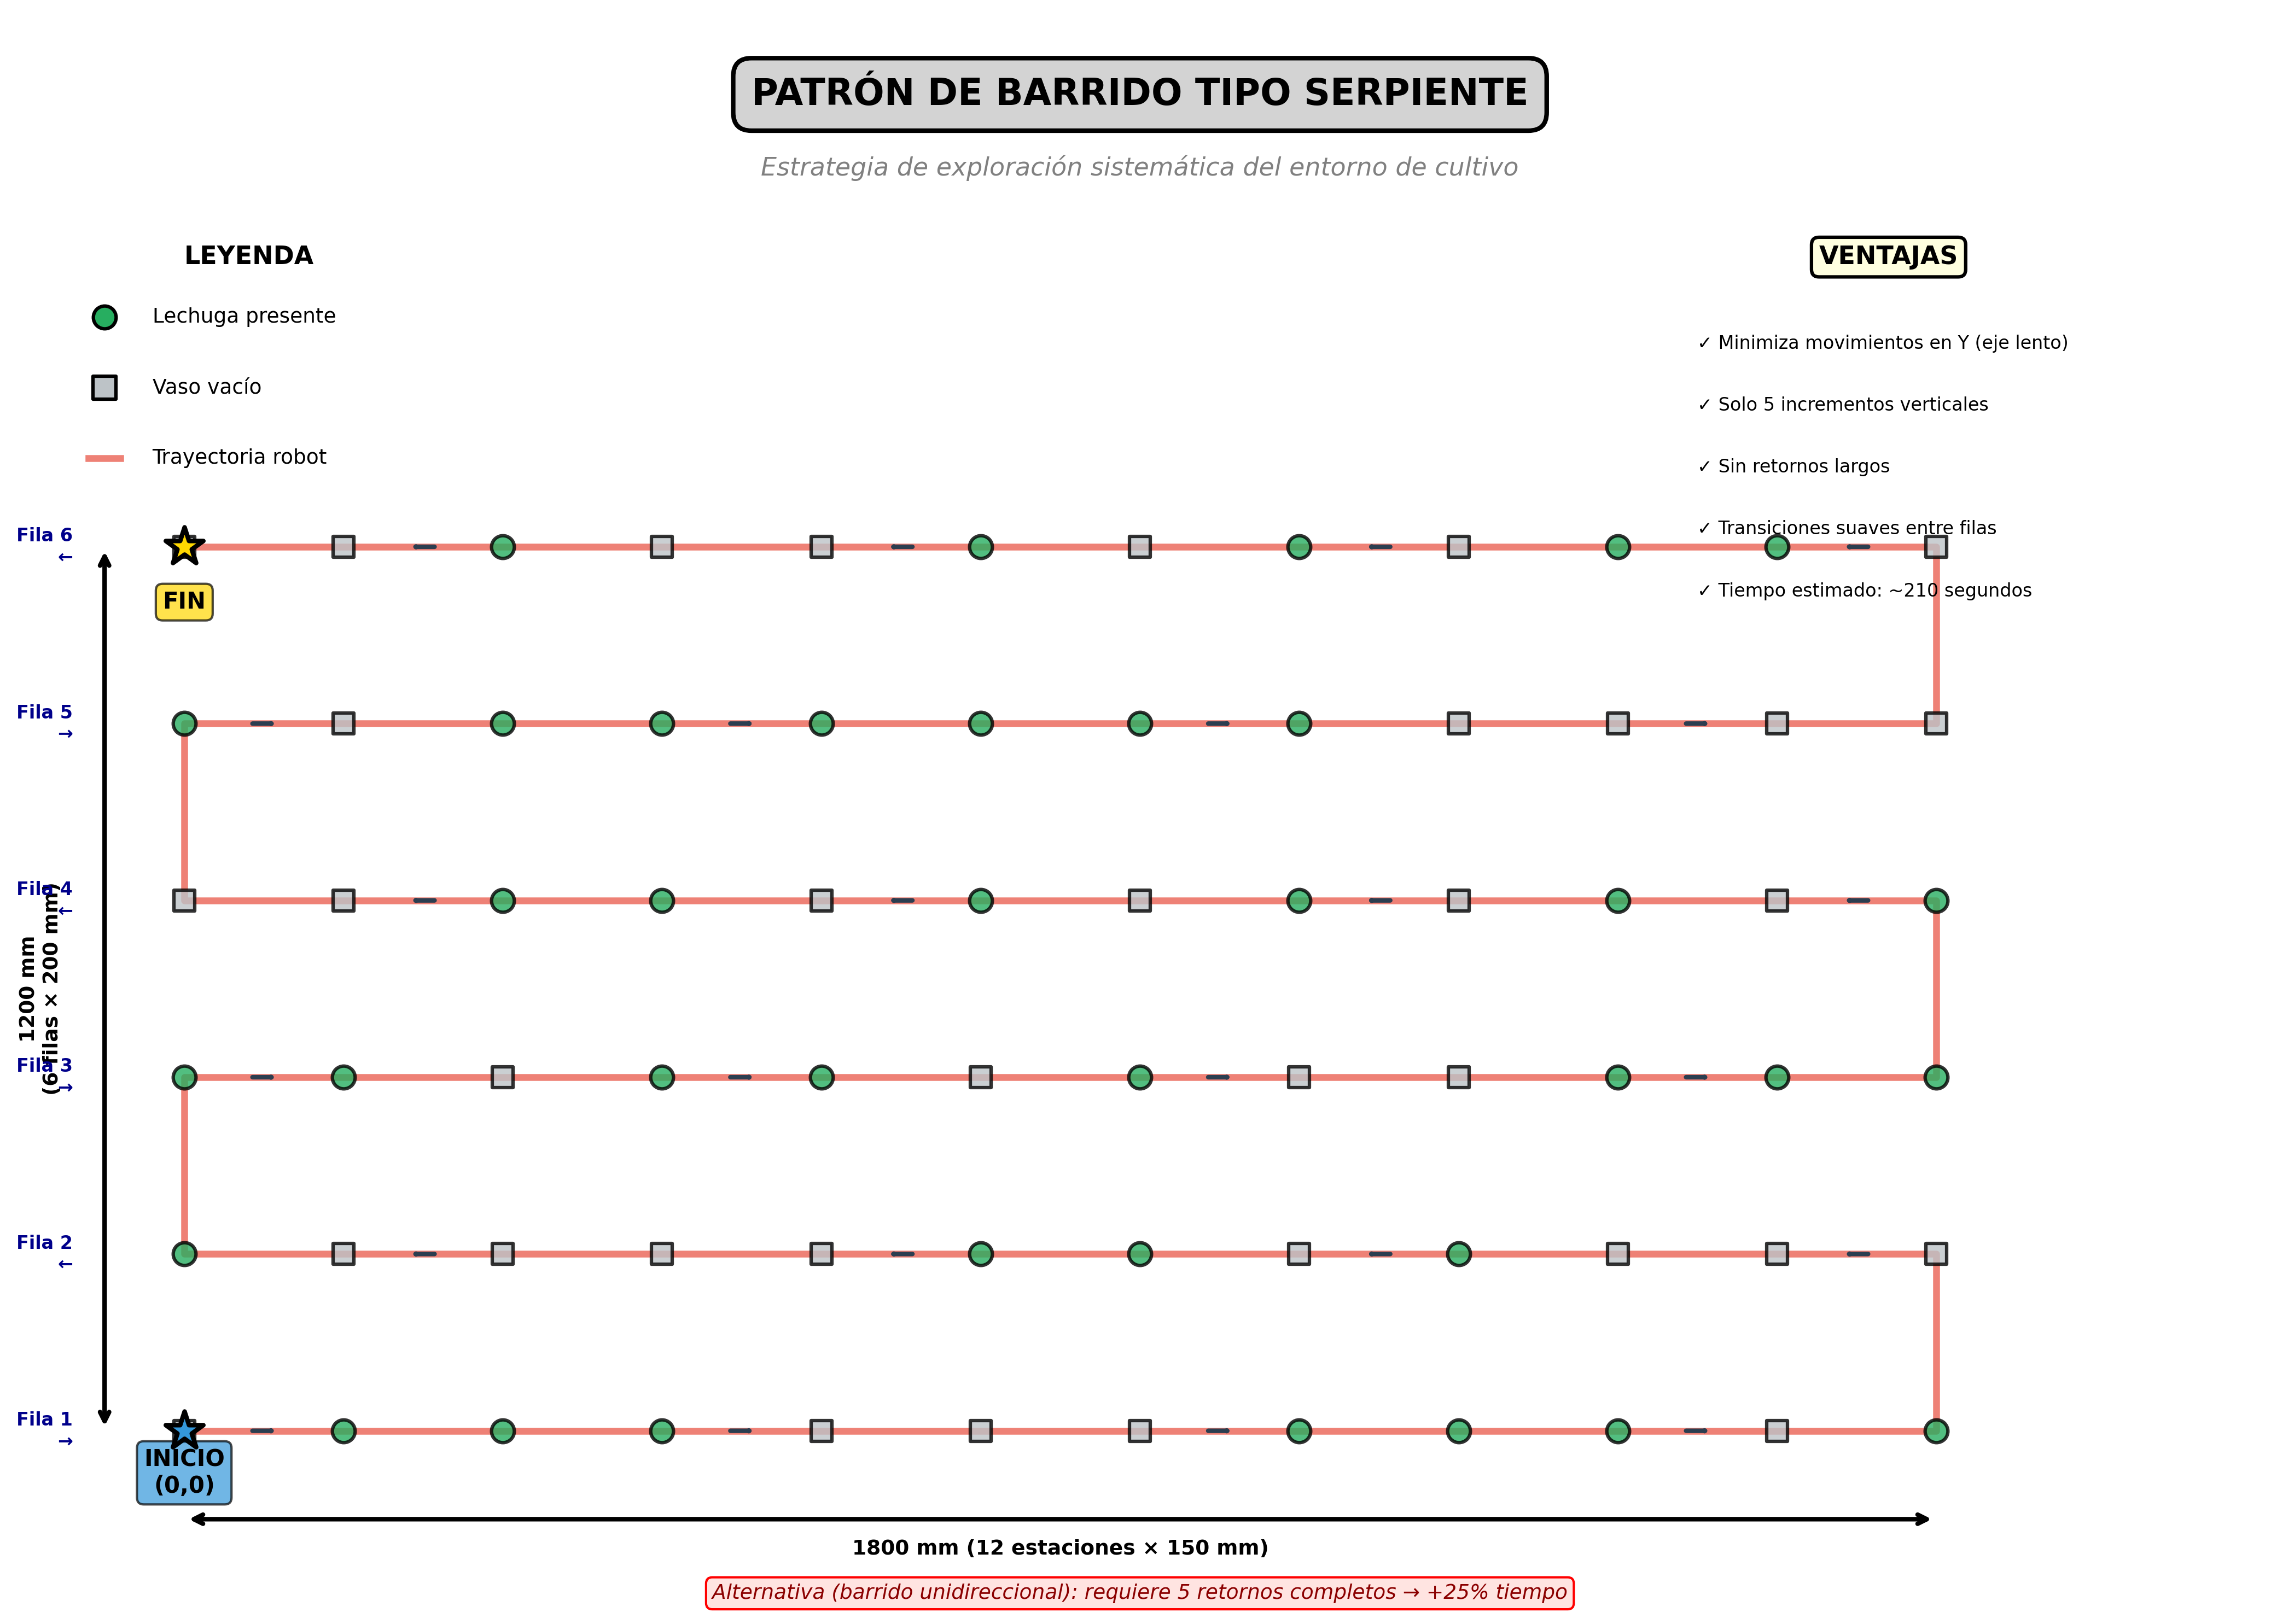
\includegraphics[width=0.8\textwidth]{imagenes/patron_barrido_serpiente.png}
\caption{Patrón de barrido tipo serpiente implementado para exploración del entorno de cultivo}
\label{fig:patron_barrido}
\end{figure}

La ventaja de este patrón es doble. Primero, minimiza el número de movimientos en el eje lento (vertical): solamente se requieren 5 incrementos de posición en Y para completar las 6 filas, en contraste con el patrón de barrido unidireccional que requeriría retornos largos tras cada fila. Segundo, elimina movimientos largos de retorno: cada fila termina en la posición donde inicia la siguiente fila, resultando en transiciones suaves entre filas.

El tiempo estimado de exploración completa se calcula considerando el número de estaciones, el tiempo de desplazamiento entre estaciones adyacentes y el tiempo de procesamiento en cada estación. Para 72 estaciones con tiempo promedio de 2.5 segundos por movimiento horizontal, 0.3 segundos de estabilización y 0.15 segundos de clasificación, el tiempo total es de aproximadamente 210 segundos, equivalente a 3.5 minutos.

\subsubsection{Sincronización entre Visión y Movimiento}

Para garantizar la calidad de las imágenes capturadas es imperativo que el robot se encuentre completamente estático durante la adquisición. El movimiento durante la captura genera desenfoque que degrada significativamente la precisión de la detección y clasificación. Se implementó un protocolo de sincronización estricto entre el nivel supervisor (Raspberry Pi) y el nivel regulatorio (Arduino).

La secuencia de operaciones en cada estación se estructura como sigue. Primero, el nivel supervisor calcula las coordenadas objetivo de la próxima estación y transmite un comando de movimiento al Arduino mediante comunicación UART. El comando especifica las coordenadas absolutas destino. El Arduino ejecuta el movimiento coordinado de los motores paso a paso y, al finalizar, transmite un mensaje de confirmación al supervisor indicando que el desplazamiento se completó.

El supervisor, al recibir la confirmación, implementa una pausa de estabilización de 300 milisegundos. Esta pausa es necesaria para permitir la disipación de vibraciones mecánicas residuales del sistema. Las vibraciones, aunque pequeñas, pueden causar desplazamiento de píxeles en la imagen que afectan la precisión de la detección de contornos. Mediciones experimentales mediante acelerómetro revelaron que las vibraciones se atenúan por debajo del umbral de detección visual en aproximadamente 250 milisegundos, estableciéndose 300 milisegundos como margen de seguridad.

Tras la estabilización, el supervisor ejecuta el algoritmo de corrección de posición visual descrito en la sección anterior. Este paso garantiza que el robot se encuentra precisamente alineado frente a la estación objetivo, compensando cualquier error acumulado durante los desplazamientos previos. Finalmente, con el robot correctamente posicionado y estático, se ejecuta la captura de imagen y el pipeline de clasificación.

El protocolo de comunicación entre niveles emplea mensajes de texto ASCII terminados en carácter de nueva línea. El supervisor transmite comandos con formato estructurado que incluye identificador de operación y parámetros numéricos. Por ejemplo, el comando para mover a la coordenada (150, 200) se codifica como la cadena de texto que especifica la operación y las coordenadas. El Arduino procesa el comando, ejecuta la acción y responde con un mensaje de estado que indica finalización exitosa o código de error si aplicable.

Esta sincronización garantiza que las capturas se realizan consistentemente bajo condiciones óptimas, maximizando la confiabilidad del sistema de clasificación.

\subsubsection{Mecanismo de Cooldown Espacial}

Un desafío potencial del sistema de mapeo es la posibilidad de procesar la misma estación múltiples veces debido a pequeñas variaciones en el posicionamiento del robot. Si el robot se posiciona con un error de ±5 milímetros cerca del límite entre dos estaciones adyacentes, podría capturar la misma estación desde posiciones ligeramente diferentes en momentos distintos, resultando en entradas duplicadas en el mapa.

Para prevenir este problema se implementó un mecanismo de cooldown espacial que mantiene un registro de las estaciones ya procesadas. Antes de clasificar una estación, el sistema verifica si existe una entrada previa en el registro cuya posición se encuentra dentro de un radio de tolerancia de la posición actual. Si existe tal entrada, el sistema omite el procesamiento y avanza a la siguiente estación.

La verificación se realiza calculando la distancia euclidiana entre la posición actual y cada posición registrada previamente:

\begin{equation}
d = \sqrt{(x_{actual} - x_{previo})^2 + (y_{actual} - y_{previo})^2}
\end{equation}

Si esta distancia es inferior a un umbral de tolerancia de 50 milímetros, se considera que ambas posiciones corresponden a la misma estación. Este valor de umbral se seleccionó considerando que la separación mínima entre estaciones es de 150 milímetros, garantizando que estaciones distintas no se confundan mientras se tolera la variabilidad de posicionamiento del robot.

El registro de posiciones procesadas se implementa como una lista dinámica que crece durante la exploración. Para cada estación procesada exitosamente, sus coordenadas se agregan al registro. La búsqueda en el registro se realiza secuencialmente, operación que presenta complejidad temporal lineal en el número de estaciones procesadas. Dado que el número máximo de estaciones es 72, esta complejidad es aceptable y no impacta significativamente el tiempo total de exploración.

\subsubsection{Estructura de Datos del Mapa}

Los resultados del proceso de mapeo se almacenan en una estructura de datos que facilita consultas posteriores y planificación de trayectorias. La estructura fundamental es una matriz donde cada fila representa una estación de cultivo y contiene tres elementos: coordenada X en milímetros, coordenada Y en milímetros, y estado de la estación.

El estado de cada estación se codifica mediante valores enteros: 0 indica vaso vacío sin lechuga, 1 indica lechuga presente disponible para cosecha, y 2 indica estación ya cosechada. Esta última categoría se emplea durante la fase de cosecha para marcar estaciones que inicialmente contenían lechuga pero ya fueron procesadas.

Matemáticamente, el mapa se representa como:

\begin{equation}
\mathbf{M}_{cultivo} = \begin{bmatrix}
x_1 & y_1 & e_1 \\
x_2 & y_2 & e_2 \\
\vdots & \vdots & \vdots \\
x_n & y_n & e_n
\end{bmatrix}
\end{equation}

donde $n$ es el número total de estaciones exploradas, $(x_i, y_i)$ son las coordenadas de la estación $i$, y $e_i \in \{0, 1, 2\}$ es su estado.

La implementación emplea arrays de NumPy que proporcionan operaciones eficientes de búsqueda y filtrado. Por ejemplo, obtener todas las estaciones con lechuga disponible se realiza mediante indexación booleana, filtrando las filas donde la tercera columna es igual a 1. Esta operación es computacionalmente eficiente y presenta complejidad temporal lineal en el número de estaciones.

Durante la exploración, cada vez que se procesa una estación nueva, se agrega una fila al mapa con las coordenadas actuales y el resultado de la clasificación. Al finalizar la exploración, el mapa contiene la representación completa del entorno, con típicamente 72 entradas para un sistema completo.

\subsubsection{Actualización Dinámica durante Cosecha}

El mapa no es estático sino que se actualiza dinámicamente durante la fase de cosecha. Cuando el robot completa exitosamente la cosecha de una lechuga, el sistema busca en el mapa la entrada correspondiente a esa posición y actualiza su estado de 1 (lechuga disponible) a 2 (ya cosechada).

La búsqueda de la entrada correspondiente se realiza identificando la fila cuyas coordenadas X e Y se encuentran dentro de una tolerancia de 20 milímetros de la posición donde se ejecutó la cosecha. Esta tolerancia contempla pequeñas variaciones entre la posición registrada durante el mapeo y la posición alcanzada durante la cosecha.

La actualización del estado es crítica para evitar que el robot intente cosechar nuevamente una estación ya procesada si, por alguna razón, el sistema reinicia o ejecuta un segundo ciclo de operación. También proporciona información valiosa para análisis post-operación, permitiendo generar estadísticas de rendimiento como número de lechugas cosechadas, tasa de éxito de cosecha, y distribución espacial de cultivos.

\subsubsection{Persistencia de Datos}

Para permitir recuperación ante fallos y análisis posterior, el mapa se almacena periódicamente en memoria no volátil. La serialización se realiza mediante formato JSON (JavaScript Object Notation), que proporciona legibilidad humana y compatibilidad con múltiples herramientas de análisis.

El archivo JSON contiene un array de objetos donde cada objeto representa una estación con campos para coordenadas X, Y y estado. Este formato facilita la importación del mapa en software de análisis estadístico o visualización, permitiendo generar representaciones gráficas de la distribución de cultivos y patrones de cosecha.

La escritura del archivo se ejecuta tras completar la exploración y también tras cada actualización de estado durante la cosecha, con un mecanismo de escritura atómica que previene corrupción de datos en caso de interrupción abrupta de energía. El archivo se lee al inicio de cada sesión de operación, permitiendo continuar operaciones interrumpidas o analizar datos históricos.

El tamaño del archivo es reducido (típicamente menos de 5 kilobytes para 72 estaciones), permitiendo almacenamiento de múltiples sesiones sin comprometer el espacio disponible en la tarjeta microSD de la Raspberry Pi. Los archivos se nombran con marca temporal que incluye fecha y hora de la sesión, facilitando su organización y recuperación.